% =====================================================================
% Como o WitnessRAG funciona: explicação passo a passo
% Compilar: latexmk -pdf witnessrag-explicado.tex
% =====================================================================
\documentclass[11pt]{article}
\usepackage[margin=2.4cm]{geometry}
\usepackage[T1]{fontenc}
\usepackage[utf8]{inputenc}
\usepackage[brazilian, provide=*]{babel}
\usepackage{amsmath,amssymb,amsthm}
\usepackage{booktabs,tabularx,array}
\usepackage{enumitem}
\usepackage{xcolor}
\usepackage[most]{tcolorbox}
\usepackage{tikz}
\usetikzlibrary{arrows.meta,positioning,fit,backgrounds,shapes.geometric,calc,decorations.pathreplacing}
\usepackage[hidelinks]{hyperref}

\newtheorem{definicao}{Definição}
\newtheorem{propriedade}{Propriedade}
\AtBeginDocument{\renewcommand{\proofname}{Por quê}}

\newtcolorbox{ideia}{enhanced, breakable, colback=blue!3, colframe=blue!45!black,
  title=A ideia, fonttitle=\bfseries\sffamily, boxrule=0.5pt, arc=2pt}
\newtcolorbox{exemplo}[1][]{enhanced, breakable, colback=green!3, colframe=green!40!black,
  title={Exemplo#1}, fonttitle=\bfseries\sffamily, boxrule=0.5pt, arc=2pt}
\newtcolorbox{cuidado}{enhanced, breakable, colback=red!3, colframe=red!45!black,
  title=Cuidado, fonttitle=\bfseries\sffamily, boxrule=0.5pt, arc=2pt}
\newtcolorbox{resumo}{enhanced, breakable, colback=gray!5, colframe=gray!60,
  coltitle=black, title=Para guardar, fonttitle=\bfseries\sffamily, boxrule=0.4pt, arc=2pt}

\newcommand{\Compose}{\textsc{Compor}}
\newcommand{\Direct}{\textsc{Direta}}
\tikzset{
  box/.style={draw, rounded corners=2pt, align=center, minimum height=7mm, inner sep=3pt, fill=white, font=\sffamily\footnotesize},
  llm/.style={box, fill=blue!7},
  sym/.style={box, fill=green!7},
  dec/.style={draw, diamond, aspect=2.2, align=center, inner sep=1pt, fill=yellow!10, font=\sffamily\footnotesize},
  arr/.style={-{Latex[length=2mm]}, thick},
  ent/.style={draw, circle, minimum size=12mm, align=center, font=\sffamily\footnotesize, fill=white},
}

\title{\textbf{Como o WitnessRAG funciona}\\[2pt]\large Uma explicação passo a passo}
\author{}
\date{23 de setembro de 2026}

\begin{document}
\maketitle
\tableofcontents

% =====================================================================
\section{Resumo de como funciona}\label{sec:resumo}

O WitnessRAG é uma memória para agentes que conversam durante muito tempo.
Quando alguém faz uma pergunta sobre o passado, ele precisa escolher poucos
trechos da conversa (cinco páginas) para entregar a um modelo de linguagem,
que então responde. Todo o método é uma resposta para a pergunta ``quais
cinco páginas?''.

A resposta do WitnessRAG é: \emph{as páginas que demonstram a resposta}. Em
vez de escolher trechos só porque se parecem com a pergunta, ele tenta
encontrar uma \textbf{testemunha}: um conjunto mínimo de fatos guardados que,
juntos, provam a resposta. As páginas de onde esses fatos vieram são as que
vale a pena mostrar.

O processo tem duas partes, como no GAM (General Agentic Memory):

\begin{enumerate}[leftmargin=*]
\item \textbf{Antes de qualquer pergunta} (o \emph{memorizador}): a conversa
inteira é guardada em páginas, cada fala recebe a sua data, expressões como
``ontem'' viram datas absolutas, e um modelo de linguagem extrai fatos no
formato (sujeito, relação, objeto, tempo), que formam um grafo.
\item \textbf{A cada pergunta} (o \emph{pesquisador}):
\begin{enumerate}[label=(\alph*), nosep]
\item faz uma busca híbrida (por significado e por palavras) e separa as 5
melhores páginas: esse é o contexto de reserva;
\item escreve um pequeno \emph{plano} (o contrato de evidência) dizendo o
que a pergunta pede;
\item decide, pelo plano, se a pergunta admite uma testemunha;
\item se admite, traduz a pergunta numa consulta lógica, procura testemunhas
no grafo e, se encontrar uma boa, coloca as páginas dela no fim do contexto;
\item entrega as 5 páginas a um leitor, que responde.
\end{enumerate}
\end{enumerate}

\begin{figure}[h]
\centering
\resizebox{\textwidth}{!}{%
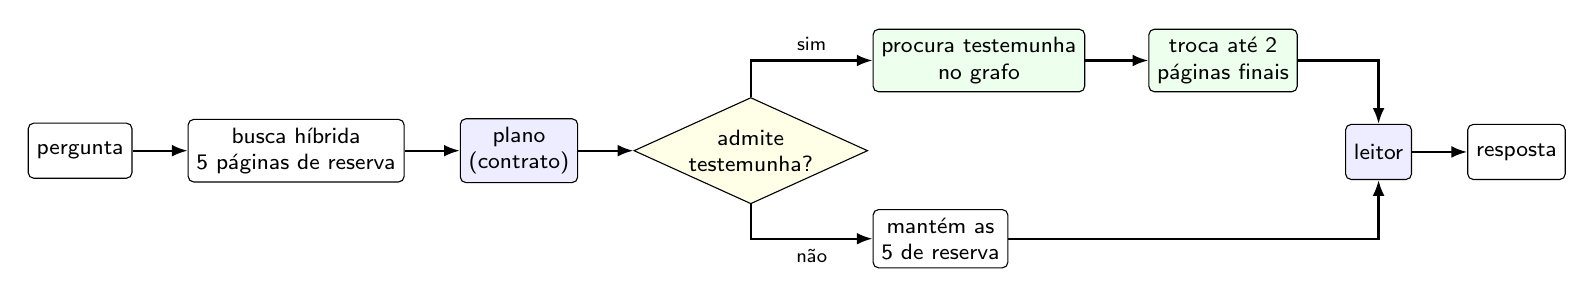
\begin{tikzpicture}[node distance=5mm and 7mm]
\node[box] (q) {pergunta};
\node[box, right=of q] (hyb) {busca híbrida\\5 páginas de reserva};
\node[llm, right=of hyb] (plan) {plano\\(contrato)};
\node[dec, right=of plan] (d) {admite\\testemunha?};
\node[sym, above right=4mm and 8mm of d] (comp) {procura testemunha\\no grafo};
\node[box, below right=4mm and 8mm of d] (dir) {mantém as\\5 de reserva};
\node[sym, right=8mm of comp] (ins) {troca até 2\\páginas finais};
\node[llm, below right=4mm and 6mm of ins] (read) {leitor};
\node[box, right=of read] (a) {resposta};
\draw[arr] (q) -- (hyb); \draw[arr] (hyb) -- (plan); \draw[arr] (plan) -- (d);
\draw[arr] (d) |- node[above, pos=0.75, font=\sffamily\scriptsize]{sim} (comp);
\draw[arr] (d) |- node[below, pos=0.75, font=\sffamily\scriptsize]{não} (dir);
\draw[arr] (comp) -- (ins);
\draw[arr] (ins) -| (read);
\draw[arr] (dir) -| (read);
\draw[arr] (read) -- (a);
\end{tikzpicture}}
\caption{O caminho de uma pergunta, em uma figura. Azul: chamadas ao modelo
de linguagem. Verde: passos lógicos, sem modelo.}
\label{fig:resumo}
\end{figure}

\begin{resumo}
\begin{itemize}[nosep, leftmargin=*]
\item \textbf{Testemunha em vez de semelhança}: o que entra no contexto é o
que demonstra a resposta, não só o que se parece com a pergunta.
\item \textbf{Plano em vez de rótulo}: o sistema entende sozinho o que a
pergunta pede; não usa a categoria do benchmark.
\item \textbf{Mexer pouco}: o sistema parte de uma busca forte e troca no
máximo duas das cinco páginas. Um erro custa pouco.
\item \textbf{Custo}: 2 chamadas ao modelo por pergunta (plano e leitura), ou
3 quando procura testemunha (mais a tradução para consulta lógica).
\end{itemize}
\end{resumo}

% =====================================================================
\section{O que é uma testemunha}\label{sec:testemunha}

\begin{ideia}
Pense num julgamento. O veredito não se apoia em ``tudo o que foi dito
parecido com o caso'', e sim num conjunto de provas que, juntas, sustentam a
conclusão. Uma testemunha, aqui, é exatamente isso: as peças mínimas de
informação que, juntas, provam uma resposta. Tire uma peça e a prova cai.
\end{ideia}

\subsection{Um exemplo pequeno}

Suponha que a memória tenha cinco fatos:

\begin{center}
\begin{tabular}{cl}
$e_1$ & Ana trabalha na Atlas \\
$e_2$ & Atlas fica em Recife \\
$e_3$ & Ana pesquisa Óptica \\
$e_4$ & Bruno trabalha na Atlas \\
$e_5$ & Bruno pesquisa Óptica \\
\end{tabular}
\end{center}

\textbf{Pergunta 1:} ``Em que cidade fica o empregador da Ana?'' Nenhum fato
sozinho responde. É preciso dois passos: descobrir onde a Ana trabalha
($e_1$: Atlas) e depois onde a Atlas fica ($e_2$: Recife). A testemunha da
resposta ``Recife'' é $\{e_1,e_2\}$. Os dois fatos são necessários: sem $e_1$
não se sabe qual empresa; sem $e_2$ não se sabe a cidade.

\textbf{Pergunta 2:} ``Quem trabalha na Atlas e pesquisa Óptica?'' Aqui a
\emph{mesma} pessoa precisa cumprir as duas condições. Há duas respostas, cada
uma com a sua testemunha: Ana, com $\{e_1,e_3\}$, e Bruno, com $\{e_4,e_5\}$.
Um conjunto como $\{e_1,e_5\}$ \emph{não} é testemunha de nada: ele mostra
alguém da Atlas (Ana) e alguém que pesquisa Óptica (Bruno), mas não a mesma
pessoa. Essa é a diferença entre ``trechos relevantes'' e ``prova''.

\begin{figure}[h]
\centering
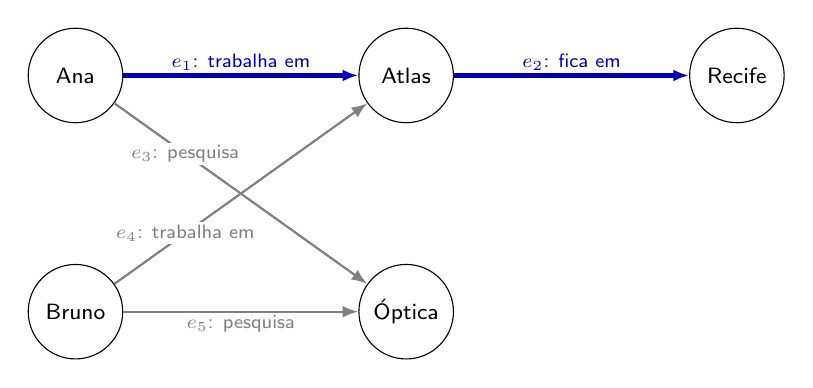
\begin{tikzpicture}[lbl/.style={font=\sffamily\scriptsize, fill=white, inner sep=1pt}]
\node[ent] (ana) at (0,0) {Ana};
\node[ent] (atlas) at (4.2,0) {Atlas};
\node[ent] (recife) at (8.4,0) {Recife};
\node[ent] (bruno) at (0,-3) {Bruno};
\node[ent] (optica) at (4.2,-3) {Óptica};
\draw[arr, blue!70!black, line width=1.6pt] (ana) -- node[above, lbl]{$e_1$: trabalha em} (atlas);
\draw[arr, blue!70!black, line width=1.6pt] (atlas) -- node[above, lbl]{$e_2$: fica em} (recife);
\draw[arr, gray] (ana) -- node[pos=0.28, lbl]{$e_3$: pesquisa} (optica);
\draw[arr, gray] (bruno) -- node[pos=0.28, lbl]{$e_4$: trabalha em} (atlas);
\draw[arr, gray] (bruno) -- node[below, lbl]{$e_5$: pesquisa} (optica);
\end{tikzpicture}
\caption{Em azul, a testemunha $\{e_1,e_2\}$ da resposta ``Recife'' à
pergunta 1. Os demais fatos existem na memória, mas não fazem parte desta
prova.}
\label{fig:testemunha}
\end{figure}

\subsection{A definição}

Para falar disso com precisão, escrevemos a pergunta como uma
\emph{consulta conjuntiva}: uma lista de condições ligadas por ``e'', com
variáveis para o que ainda não se sabe.
\[
Q_1(x)=\exists y\;\ \mathrm{trabalhaEm}(\text{Ana},y)\ \wedge\ \mathrm{ficaEm}(y,x).
\]
Lê-se: ``$x$ é resposta se existe algum $y$ tal que Ana trabalha em $y$
\emph{e} $y$ fica em $x$''. Cada condição é um \emph{átomo}. A variável $y$ é
intermediária (a empresa); $x$ é a resposta (a cidade).

\begin{definicao}[Testemunha]
Dada uma memória de fatos $F$, uma consulta $Q$ e uma resposta $a$, uma
testemunha de $a$ é um conjunto $W\subseteq F$ tal que
(i) os fatos de $W$ bastam para demonstrar que $a$ responde $Q$, e
(ii) nenhum subconjunto próprio de $W$ basta.
Escrevemos $\mathcal{W}_{Q,a}$ para o conjunto de todas as testemunhas de $a$.
\end{definicao}

A condição (ii) é a \emph{minimalidade}: nada sobra na prova. Note que
``mínima'' não quer dizer ``a menor possível'': uma resposta pode ter várias
testemunhas diferentes, de tamanhos diferentes, todas mínimas no sentido de
que nenhum fato delas é dispensável.

\subsection{A propriedade que justifica o método}

\begin{propriedade}
Uma resposta $a$ pode ser obtida de uma memória $S$ se, e somente se, pelo
menos uma testemunha de $a$ está inteira dentro de $S$:
\[
a\in\mathrm{Ans}(Q,S)\iff\exists\,W\in\mathcal{W}_{Q,a}\ \text{com}\ W\subseteq S.
\]
\end{propriedade}
\begin{proof}
Se uma testemunha inteira está em $S$, os seus fatos demonstram a resposta, e
fatos a mais não atrapalham (as condições são todas positivas, do tipo ``e'').
Se a resposta sai de $S$, existe uma escolha de valores para as variáveis que
torna cada condição verdadeira por algum fato de $S$; tirando os fatos que
sobram, chega-se a uma testemunha dentro de $S$.
\end{proof}

A consequência é direta: \textbf{guardar e recuperar respostas é o mesmo que
guardar e recuperar testemunhas}. Se o contexto entregue ao leitor contém uma
testemunha inteira, a informação necessária para responder está lá.

\subsection{Várias testemunhas: o ``ou'' de ``e''s}

Se uma resposta tem várias testemunhas, qualquer uma delas serve. Isso dá a
cada resposta uma fórmula de ``ou'' de ``e''s, chamada \emph{polinômio de
proveniência}:
\[
\text{Ana}\ \Leftarrow\ (e_1\wedge e_3)\ \vee\ (\text{outra prova, se houver}).
\]
Cada termo entre parênteses é uma testemunha. Isso explica por que duplicar a
mesma prova não deve aumentar a confiança numa resposta: o WitnessRAG usa a
força da \emph{melhor} testemunha, não a soma de todas.

\subsection{Respostas que são conjuntos}

\begin{exemplo}[ real do LoCoMo: ``Where has Melanie camped?'']
Resposta de referência: \emph{beach, mountains, forest}. Os três itens
aparecem em três sessões diferentes:
\begin{itemize}[nosep]
\item 27/6/2023: ``\dots I just took my fam camping in the mountains last week\dots''
\item 6/7/2023: ``\dots Here's a pic of my family camping at the beach\dots''
\item 15/7/2023: ``\dots We even went on another camping trip in the forest.''
\end{itemize}
A consulta é $Q(x)=\mathrm{acampou}(\text{Melanie},x)$ e a resposta é o
\emph{conjunto} de todos os $x$ com testemunha. Cada membro tem a sua própria
testemunha de um fato: $\{f_{\text{montanhas}}\}$, $\{f_{\text{praia}}\}$,
$\{f_{\text{floresta}}\}$. Uma busca por semelhança costuma trazer uma ou
duas dessas falas; a lógica de conjunto força a procurar todas.
\end{exemplo}

\subsection{Testemunha não é ``trecho relevante''}

Um trecho relevante \emph{se parece} com a pergunta. Uma testemunha
\emph{basta} para a resposta. As duas coisas não coincidem: o segundo elo de
uma cadeia (``Atlas fica em Recife'') não se parece nada com a pergunta
``Onde fica o empregador da Ana?'', porque não menciona a Ana, e mesmo assim é
indispensável. É justamente o tipo de trecho que a busca por semelhança perde.

\begin{cuidado}
Três limites honestos. (1) A testemunha só existe se o extrator registrou os
fatos; um fato não extraído não pode ser provado. (2) Os fatos são casados
com a consulta por similaridade (``camp in'' casa com ``acampou''), então na
prática a testemunha é uma testemunha \emph{candidata}, não um certificado
absoluto; por isso o leitor sempre lê o texto original das páginas. (3) Para
respostas-conjunto, a completude não é garantida: o conjunto contém o que a
memória prova, e nada impede que um item tenha ficado de fora na extração.
\end{cuidado}

% =====================================================================
\section{Formulação do problema}\label{sec:problema}

\begin{ideia}
O problema não é ``responder perguntas''; é \emph{escolher o contexto}.
O leitor é o mesmo para todos os métodos; o que muda é o que ele recebe.
\end{ideia}

\paragraph{O que é dado.}
Um histórico de conversa $H=(s_1,\dots,s_T)$, dividido em sessões; cada fala
$u$ tem um locutor, um texto e a data da sessão, $\tau(u)$. Uma pergunta $q$.
Um orçamento de contexto de $k=5$ páginas.

\paragraph{O que é pedido.}
Um contexto $C(q)$, com exatamente $k$ páginas, tal que o leitor
$\mathrm{Read}(q,C(q))$ acerte o máximo possível:
\[
C^\star(q)\in\arg\max_{|C|=k}\ \mathbb{E}\bigl[\Gamma(\mathrm{Read}(q,C))\bigr],
\]
em que $\Gamma$ é a métrica (por exemplo, F1). Em palavras: entre todos os
conjuntos de 5 páginas, queremos o que faz o leitor acertar mais.

\paragraph{As restrições.}
\begin{itemize}[nosep]
\item \textbf{Poucas chamadas}: no máximo 3 chamadas ao modelo por pergunta.
\item \textbf{Sem rótulos}: o sistema não pode saber a categoria da pergunta
(``multi-hop'', ``temporal''\dots); em produção isso não existe.
\item \textbf{Sem gabarito}: nenhuma etapa vê a resposta correta nem as falas
de apoio anotadas.
\item \textbf{Mesmo leitor}: para que a comparação entre métodos meça
recuperação, e não engenharia de prompt.
\end{itemize}

\paragraph{Por que é difícil.}
Resumir a conversa antes perde detalhes (o problema do ``ahead of time''
apontado pelo GAM). Buscar por semelhança perde os elos que não se parecem com
a pergunta. E o orçamento é apertado: uma conversa do LoCoMo tem de 7 a 13
páginas, e só 5 podem ser mostradas. Escolher errado uma única página pode
tirar do leitor o fato decisivo.

\paragraph{Como o WitnessRAG quebra o problema.}
Em cinco subproblemas, cada um com a sua ferramenta:
\begin{center}
\small
\begin{tabularx}{\textwidth}{@{}l>{\raggedright\arraybackslash}X@{}}
\toprule
Subproblema & Ferramenta \\
\midrule
O que a pergunta pede? & o contrato de evidência (uma chamada ao modelo) \\
Existe prova possível? & a regra de roteamento (lógica, sem modelo) \\
Qual é a prova? & compilação + junção no grafo de fatos \\
Como caber em 5 páginas sem estragar? & edição de no máximo 2 posições da busca híbrida \\
Qual é a resposta? & um leitor único, que lê o texto original \\
\bottomrule
\end{tabularx}
\end{center}

% =====================================================================
\section{Como a memória é construída}\label{sec:memoria}

\begin{ideia}
A memória guarda a mesma conversa de duas formas: o \textbf{texto integral},
para ler, e \textbf{fatos estruturados}, para raciocinar. Os fatos servem
para \emph{encontrar} a prova; o texto serve para \emph{responder}. Nada é
resumido e nada é jogado fora.
\end{ideia}

\subsection{Páginas com relógio}

A conversa é cortada em páginas de até 2.048 tokens (o mesmo tamanho usado
pelo GAM). Cada página começa com a data da sessão, e cada fala carrega a sua
data, o \emph{relógio de referência} $\tau(u)$. Isso é importante porque as
pessoas falam do tempo de forma relativa (``ontem'', ``semana passada''), e
essas expressões só fazem sentido em relação ao dia em que foram ditas.

Por isso, antes de qualquer pergunta, um normalizador simples (regras de
calendário, sem modelo) escreve ao lado de cada fala o valor absoluto dessas
expressões. Um trecho real:

\begin{quote}\small\ttfamily
Session date: 1:56 pm on 8 May, 2023\\
{[D1:3]} Caroline: I went to a LGBTQ support group yesterday and it was so powerful.\\
{[D1:3 temporal]} reference\_time=2023-05-08; "yesterday"=7 May 2023
\end{quote}

A fala original não é alterada; a anotação fica ao lado. Quando alguém
perguntar ``When did Caroline go to the LGBTQ support group?'', a resposta
(7 May 2023) já está escrita na página.

\subsection{Fatos extraídos}

Um modelo de linguagem lê a conversa em janelas de 512 tokens e extrai fatos
no formato (sujeito, relação, objeto, tempo). Em diálogo, isso exige cuidados
que o extrator segue:
\begin{itemize}[nosep]
\item ``eu'', ``meu'' viram o nome de quem fala;
\item parentes e objetos são nomeados pelo dono (``a avó da Caroline'');
\item a relação é curta e reutilizável (``read'', ``work at'', ``child of'');
\item o fato é sobre o \emph{conteúdo} da fala, não sobre quem ouviu;
\item o tempo entra como quarto elemento.
\end{itemize}

\begin{exemplo}[ (o exemplo sintético que o próprio prompt usa)]
\begin{quote}\small\ttfamily
Session date: 8 May, 2023\\
{[D1:1]} Ravi: I finally finished The Secret Garden with my son Niko last week!\\
{[D1:2]} Lea: Nice! I painted a sunset yesterday.
\end{quote}
vira os fatos
(Ravi, read, The Secret Garden, last week),
(Niko, child of, Ravi, --) e
(Lea, paint, a sunset, 7 May 2023).
\end{exemplo}

Cada fato guarda de qual página veio. É essa ligação que permite, mais tarde,
ir da testemunha (fatos) de volta ao texto (páginas).

\subsection{Identidade e vocabulário}

Para que a lógica funcione, a mesma coisa precisa ter o mesmo nome. Duas
normalizações cuidam disso: nomes parecidos que são a mesma entidade
(``Juan Courten'' e ``Juan de Courten'') são agrupados num único
\emph{cluster de identidade}; e formas da mesma relação (\emph{paint},
\emph{painted}) viram uma \emph{família}. Sem isso, uma junção quebraria por
causa de uma diferença de grafia.

\subsection{Sinais de memória}

Por fim, sem usar modelo, a memória calcula algumas estatísticas que o plano
pode querer usar depois: o relógio da conversa (primeira e última sessão),
quantas vezes cada informação foi \emph{reafirmada} em sessões diferentes,
quantas vezes cada fato foi \emph{corroborado} por extrações diferentes, e
quão emocionalmente marcante é cada fala. Esses sinais alimentam as
\emph{lentes de memória}, opcionais (Seção~\ref{sec:percurso}).

\begin{cuidado}
Nada nesta fase lê perguntas, respostas ou anotações do benchmark. A mesma
base de fatos é usada por todos os métodos baseados em grafo que comparamos
(GraphRAG, HippoRAG, HippoRAG 2), para que diferenças de resultado não sejam
diferenças de extrator.
\end{cuidado}

% =====================================================================
\section{Como uma pergunta percorre a memória}\label{sec:percurso}

\begin{ideia}
A pergunta passa por uma sequência curta de decisões. Em cada uma, se algo
dá errado, o sistema volta para o contexto de reserva (a busca híbrida). Por
isso ele pode tentar coisas ambiciosas sem arriscar muito.
\end{ideia}

\begin{figure}[h]
\centering
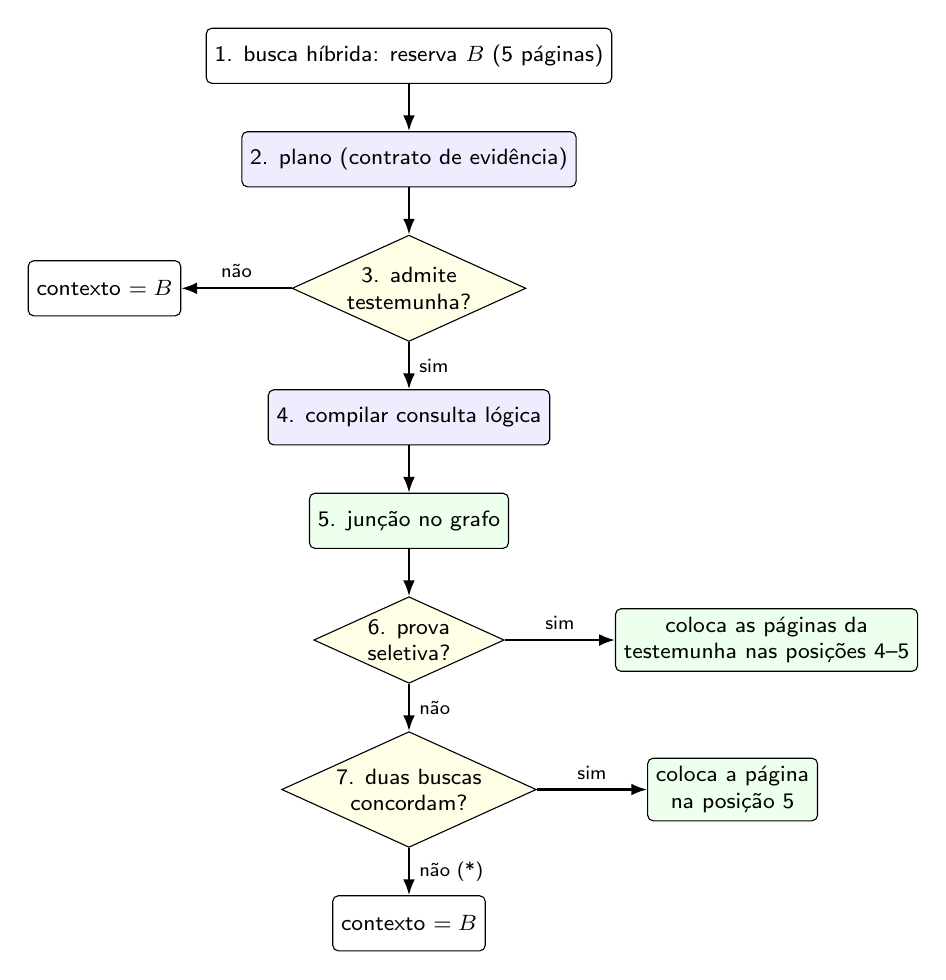
\begin{tikzpicture}[node distance=6mm and 8mm]
\node[box] (b) {1. busca híbrida: reserva $B$ (5 páginas)};
\node[llm, below=of b] (p) {2. plano (contrato de evidência)};
\node[dec, below=of p] (r) {3. admite\\testemunha?};
\node[box, left=14mm of r] (dir) {contexto $=B$};
\node[llm, below=of r] (c) {4. compilar consulta lógica};
\node[sym, below=of c] (j) {5. junção no grafo};
\node[dec, below=of j] (y) {6. prova\\seletiva?};
\node[sym, right=14mm of y] (ins) {coloca as páginas da\\testemunha nas posições 4--5};
\node[dec, below=of y] (s) {7. duas buscas\\concordam?};
\node[sym, right=14mm of s] (ins2) {coloca a página\\na posição 5};
\node[box, below=of s] (res) {contexto $=B$};
\draw[arr] (b) -- (p); \draw[arr] (p) -- (r);
\draw[arr] (r) -- node[above, font=\sffamily\scriptsize]{não} (dir);
\draw[arr] (r) -- node[right, font=\sffamily\scriptsize]{sim} (c);
\draw[arr] (c) -- (j); \draw[arr] (j) -- (y);
\draw[arr] (y) -- node[above, font=\sffamily\scriptsize]{sim} (ins);
\draw[arr] (y) -- node[right, font=\sffamily\scriptsize]{não} (s);
\draw[arr] (s) -- node[above, font=\sffamily\scriptsize]{sim} (ins2);
\draw[arr] (s) -- node[right, font=\sffamily\scriptsize]{não (*)} (res);
\end{tikzpicture}
\caption{As decisões no caminho de uma pergunta. Em todos os ramos o
resultado segue para as lentes (opcionais) e para o leitor. (*) Antes de
desistir, ainda há a sonda da lacuna, explicada no passo 7.}
\label{fig:percurso}
\end{figure}

\subsection{Os passos}

\paragraph{1. Busca híbrida (a reserva).}
A pergunta é buscada de duas formas: por significado (vetores BGE-M3) e por
palavras (BM25), e as duas listas são combinadas. As 5 primeiras páginas
formam a reserva $B$. Se nada mais der certo, o leitor recebe $B$.

\paragraph{2. Plano.}
Uma chamada ao modelo lê \emph{só o texto da pergunta} e preenche um
formulário fechado, o \emph{contrato de evidência}: que forma tem a resposta
(nome, lista, número, data, sim/não\dots), qual raciocínio vem depois da busca
(buscar um fato, juntar vários, comparar, calcular tempo, inferir), se a
resposta depende de afirmações feitas em um lugar ou em vários, se há um
período de tempo envolvido, quem são as pessoas, o que procurar, e quais
sinais de memória usar. O formulário não tem nenhuma palavra de categoria de
benchmark.

\paragraph{3. Admite testemunha? (o roteamento).}
Uma regra fixa lê o plano. A pergunta segue para a busca de testemunha
(\Compose{}) se a resposta for uma entidade ou lista de entidades e depender
de juntar, agregar ou comparar vários fatos. Caso contrário (uma data a
calcular, um ``provavelmente'', um sim/não, um fato único), fica na reserva
(\Direct{}). A lógica é: \emph{só vale procurar prova quando pode existir
prova}.

\paragraph{4. Compilar.}
Na rota \Compose{}, uma segunda chamada traduz a pergunta numa consulta
lógica, como $\mathrm{acampou}(\text{Melanie},x)$. Para evitar relações
inventadas, o modelo recebe como sugestão as relações e entidades que
realmente existem no grafo.

\paragraph{5. Junção.}
Sem modelo, o sistema procura no grafo combinações de fatos que satisfaçam
todas as condições ao mesmo tempo, com a regra de que a mesma variável tem de
receber a mesma entidade em todas as condições. Cada combinação completa é
uma testemunha.

\paragraph{6. Prova seletiva? (a reflexão).}
No GAM, um modelo de linguagem julga se a informação reunida basta. Aqui o
julgamento é lógico: a prova é aceita se existe testemunha, se a consulta não
``provou'' respostas demais (no máximo três), se não há provas duplicadas em
excesso, se a busca não foi interrompida, se os fatos casaram bem, e se a
testemunha cabe em duas páginas. Uma consulta que prova dez respostas
diferentes não está sendo seletiva, e o sistema prefere não confiar nela.

\paragraph{7. Reparo.}
Se a prova não foi aceita, há uma última tentativa, também sem modelo. As
partes da consulta viram buscas separadas; se pelo menos duas delas
concordarem numa mesma página nova, ela entra na última posição. Se a junção
parou num ponto conhecido (``achei a empresa da Ana, mas não a cidade''), o
sistema busca exatamente o que faltou. Se nada disso funcionar, fica a
reserva.

\paragraph{8. Lentes (opcionais).}
Se o plano pediu, sinais de memória podem trocar a última página: a lente
\emph{temporal} prefere o registro mais recente (``atual'', ``agora''), o
primeiro (``primeiro'') ou o mais próximo de um período citado (``em agosto
de 2023''); a lente de \emph{saliência} prefere falas emocionalmente
marcantes da pessoa em foco; a lente de \emph{confiança} prefere fatos
confirmados por várias extrações. Elas nunca tiram uma página colocada por
uma testemunha.

\subsection{Três perguntas reais}

As falas e as respostas são do LoCoMo; os planos e as consultas são
ilustrativos (o que o mecanismo faz com essas entradas).

\begin{exemplo}[ A: ``When did Caroline go to the LGBTQ support group?'']
Plano: resposta do tipo \emph{data}, raciocínio \emph{temporal}. Não admite
testemunha (é cálculo de tempo), então fica a reserva. A página certa contém
a anotação \emph{``yesterday'' = 7 May 2023}, e o leitor responde a partir
dela. \textbf{2 chamadas.}
\end{exemplo}

\begin{exemplo}[ B: ``Where has Melanie camped?'']
Plano: resposta do tipo \emph{lista}, raciocínio \emph{agregar}, evidência em
\emph{vários lugares}. Admite testemunha. Consulta:
$\mathrm{acampou}(\text{Melanie},x)$, agregação de conjunto. A junção encontra
um fato por lugar (montanhas, praia, floresta), cada um uma testemunha.
Três respostas, uma prova para cada: a prova é seletiva, e as páginas das
testemunhas entram no fim do contexto (até duas páginas; se alguma já estava
na reserva, não é repetida). \textbf{3 chamadas.}
\end{exemplo}

\begin{exemplo}[ C: ``What do Jon and Gina both have in common?'']
Resposta de referência: ambos perderam o emprego e decidiram abrir o próprio
negócio. As falas (sessão de 20/1/2023):
\begin{quote}\small
Jon: ``Lost my job as a banker yesterday, so I'm gonna take a shot at
starting my own business.''\\
Gina: ``\dots I also lost my job at Door Dash this month.''
\end{quote}
Plano: raciocínio \emph{juntar}, evidência em vários lugares: admite
testemunha. Uma consulta de interseção, ``$x$ tal que Jon perdeu $x$ e Gina
perdeu $x$'', \emph{não fecha}: os empregos são diferentes (banco e Door Dash).
O que eles têm em comum é o \emph{tipo} de acontecimento, não o mesmo objeto.
A prova não é aceita, e o reparo por buscas concordantes tende a trazer a
página da sessão 1; se ela já estava na reserva, o contexto não muda. O
leitor, lendo o texto, generaliza o que há em comum.

Este exemplo mostra por que o sistema \emph{não aposta tudo} na lógica:
quando a pergunta é mais abstrata que os fatos, a reserva híbrida e o leitor
continuam fazendo o trabalho.
\end{exemplo}

% =====================================================================
\section{Da testemunha à resposta}\label{sec:resposta}

\begin{ideia}
A testemunha decide \emph{o que mostrar}; o texto original decide \emph{a
resposta}. O leitor nunca recebe os fatos extraídos, e sim as páginas de
onde eles vieram.
\end{ideia}

\subsection{Por que entregar páginas, e não fatos}

Os fatos são uma versão comprimida da conversa: servem muito bem para
\emph{encontrar} onde está a prova, mas perdem nuance, contexto e, às vezes,
cometem erros de extração. O texto original não perde nada (é o princípio do
GAM de guardar tudo). Entregar a página resolve as duas coisas: a lógica
aponta o lugar certo, e o leitor lê o que foi realmente dito, inclusive
detalhes que o extrator não registrou.

\subsection{Como as páginas da testemunha entram no contexto}

\begin{enumerate}[nosep]
\item As respostas encontradas são ordenadas pela força da melhor
testemunha de cada uma (o produto dos casamentos dos fatos com a consulta,
ponderado pela confiança dos fatos).
\item Seguindo essa ordem, as páginas da melhor testemunha de cada resposta
são reunidas enquanto couberem em duas páginas. Testemunhas entram
\emph{inteiras}: nunca metade de uma prova.
\item As páginas que já estavam na reserva não são repetidas. As que
faltam ocupam as últimas posições (5 e depois 4). As três primeiras páginas
da busca híbrida nunca saem.
\end{enumerate}

\begin{figure}[h]
\centering
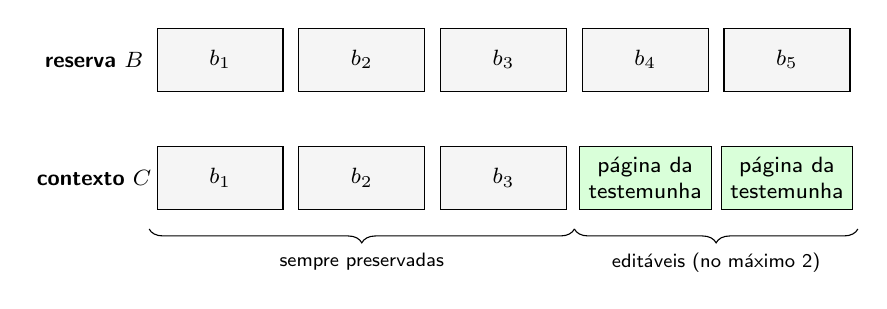
\begin{tikzpicture}[slot/.style={draw, minimum width=16mm, minimum height=8mm, font=\sffamily\footnotesize, align=center}]
\node at (-1.6,0.9) [font=\sffamily\footnotesize\bfseries] {reserva $B$};
\foreach \i/\t in {1/$b_1$,2/$b_2$,3/$b_3$,4/$b_4$,5/$b_5$}{\node[slot, fill=gray!8] (a\i) at (1.8*\i-1.8,0.9) {\t};}
\node at (-1.6,-0.6) [font=\sffamily\footnotesize\bfseries] {contexto $C$};
\foreach \i/\t in {1/$b_1$,2/$b_2$,3/$b_3$}{\node[slot, fill=gray!8] (c\i) at (1.8*\i-1.8,-0.6) {\t};}
\node[slot, fill=green!15] (c4) at (5.4,-0.6) {página da\\testemunha};
\node[slot, fill=green!15] (c5) at (7.2,-0.6) {página da\\testemunha};
\draw[decorate, decoration={brace, amplitude=5pt, mirror}] (-0.9,-1.25) -- (4.5,-1.25) node[midway, below=5pt, font=\sffamily\scriptsize]{sempre preservadas};
\draw[decorate, decoration={brace, amplitude=5pt, mirror}] (4.5,-1.25) -- (8.1,-1.25) node[midway, below=5pt, font=\sffamily\scriptsize]{editáveis (no máximo 2)};
\end{tikzpicture}
\caption{A testemunha edita no máximo as duas últimas posições do contexto de
reserva.}
\label{fig:slots}
\end{figure}

Dizemos que a testemunha \textbf{chegou ao leitor} quando todas as páginas de
pelo menos uma testemunha estão no contexto final. O sistema registra isso
para cada pergunta, junto com a rota tomada e o motivo de parada, o que
permite auditar depois por que cada resposta saiu como saiu.

\subsection{O leitor}

O mesmo leitor é usado por todas as rotas e por todos os métodos comparados.
Numa única chamada, ele:
\begin{itemize}[nosep]
\item identifica o que a pergunta pede: uma pessoa ou objeto, uma opção, uma
inferência provável, uma lista completa, uma contagem de itens distintos,
uma data, um intervalo ou uma duração;
\item exige que pessoa, evento e qualificadores venham da \emph{mesma} fala
de apoio, sem misturar menções soltas;
\item para listas, inclui todos os itens sustentados pelas páginas;
\item para tempo, usa a data da sessão da própria fala e as normalizações;
\item devolve uma resposta curta, sem explicação.
\end{itemize}
Por fim, uma normalização mínima e segura é aplicada: contagens viram
algarismos (``three'' $\to$ ``3'') e respostas de sim/não ficam no formato
curto.

\subsection{Resposta estrutural e resposta do leitor}

A junção também produz a sua própria resposta (o conjunto de respostas
testemunhadas, com a prova de cada item). Ela é registrada para auditoria,
mas \emph{não} é a resposta oficial. A oficial é a do leitor, por dois
motivos: é a única comparável entre métodos (todos usam o mesmo leitor), e o
leitor, ao ler o texto, pode corrigir o que a extração errou ou completar o
que ela deixou de fora.

\subsection{Como a resposta é avaliada, e por que listas importam}

No LoCoMo, a métrica oficial é o F1 de palavras entre a resposta e a
referência. Para perguntas de lista, a resposta é separada por vírgulas e cada
item de referência ganha o melhor casamento entre os itens respondidos:
\[
\mathrm{F1}_{\text{lista}}=\frac{1}{|G|}\sum_{g\in G}\ \max_{\hat g\in\hat G}\ \mathrm{F1}(\hat g,g),
\]
com $G$ os itens de referência e $\hat G$ os respondidos. Itens a mais não são
punidos; itens a menos, sim.

\begin{exemplo}[: o efeito de uma testemunha por item]
Referência: \emph{beach, mountains, forest}. Se o contexto só contém as falas
da praia e das montanhas, a melhor resposta possível é ``beach, mountains'',
que vale $(1+1+0)/3\approx0{,}67$. Com as três testemunhas no contexto, o
leitor pode responder os três itens e chegar a $1{,}0$. É esse ganho que a
composição busca nas perguntas de agregação.
\end{exemplo}

\subsection{O que pode dar errado em cada elo}

\begin{center}
\small
\begin{tabularx}{\textwidth}{@{}l>{\raggedright}X>{\raggedright\arraybackslash}X@{}}
\toprule
Elo & Falha possível & O que acontece \\
\midrule
extração & o fato não foi extraído & não há testemunha; fica a reserva \\
plano & rota errada & perde-se no máximo o que a outra rota mudaria (até 2 páginas) \\
compilação & relação que não existe no grafo & a junção não fecha; tenta-se o reparo \\
junção & casamento por similaridade errado & a reflexão tende a rejeitar provas amplas ou fracas \\
inserção & testemunha não cabe em 2 páginas & não é inserida; fica a reserva \\
leitura & o leitor ignora a página certa & erro do leitor, igual para todos os métodos \\
conjunto & um item nunca foi extraído & a lista sai incompleta (completude não é garantida) \\
\bottomrule
\end{tabularx}
\end{center}

\begin{resumo}
Da testemunha à resposta, o caminho é:
\emph{fatos que provam} $\to$ \emph{páginas de onde vieram} $\to$
\emph{até duas posições do contexto} $\to$ \emph{leitor que lê o texto
original} $\to$ \emph{resposta curta}. A lógica escolhe; o texto responde; e
um erro em qualquer elo custa no máximo duas das cinco páginas.
\end{resumo}

\end{document}
